\documentclass[a4]{scrartcl}

\usepackage[ngerman]{babel}
\usepackage[utf8]{inputenc}
\usepackage{mathtools}
\usepackage{amsmath}
\usepackage{adjustbox}
\usepackage{amssymb}
\usepackage{geometry}
\usepackage{scrpage2}
\pagestyle{scrheadings}
\usepackage[bottom]{footmisc}
\usepackage{footnote}
\makesavenoteenv{tabular}
\makesavenoteenv{table}
\clearscrheadfoot

\setlength{\parindent}{0em}

\geometry{
  paper=a4paper, % Change to letterpaper for US letter
  top=2cm, % Top margin
  bottom=1.5cm, % Bottom margin
  left=2cm, % Left margin
  right=3cm, % Right margin
  %showframe, % Uncomment to show how the type block is set on the page
}

\ohead{\\
Pina Kolling}


\begin{document}

\subsection*{Vorlesung 6}

\textbf{Digitale Technologien ermöglichen innovative Geschäftsideen} \\
Beispiel: Musik
\\ \\
\adjustbox{max width=\textwidth}{%

\begin{tabular}{c | c c c}

Produkt & CDs & MP$3$-Download & Streaming \\
Vertrieb & Einzelhandel & Download Plattform (Digitales Gut) & Streaming Plattform (Digitales Gut) \\
Kunde & zeitlich unbegrenzte Nutzung, & zeitlich unbegrenzte Nutzung & Nutzung durch Abonnement \\
 & Verschleiß  & & \\

\end{tabular}}

\vspace*{2em}

\textbf{Digitales Gut} 
\begin{itemize}
\item liegen in immaterieller Form vor
\item vollständig als digitale Repräsentation in Binärform gespeichert
\item können ohne Bindung an Trägermedium entwickelt, vertrieben oder angewendet werden (bsp. übers Internet)
\end{itemize}

\textbf{Digitalisierungsgrade von Gütern}

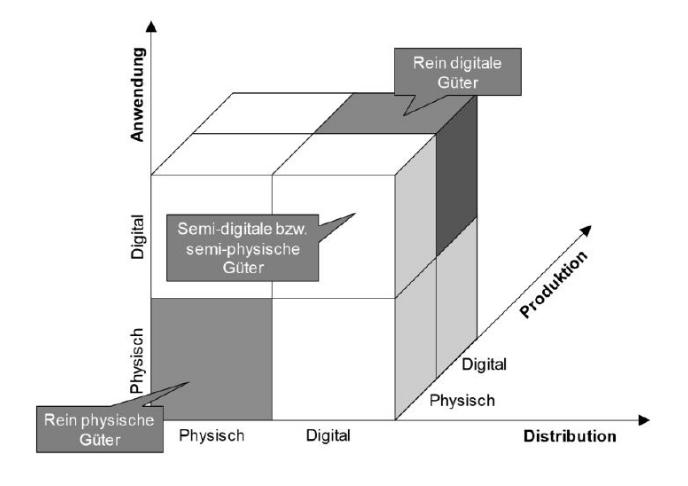
\includegraphics[scale=0.35]{wuerfel.png}

\vspace*{1em}

\textbf{Eigenschaften digitaler Güter} 

\begin{itemize}
\item Wahrnehmungsunterschiede/Interaktivität \\
Digitale Güter können nur über zwei Sinne (Sehen und Hören) wahrgenommen werden./Digitale Güter sind interaktiv vom Benutzer bedien- und steuerbar.
\item Skaleneffekte \\
Keine Kostenvorteile entstehen bei durch sinkende Kosten pro hergestelltem Produkt.
\item Kopierbarkeit/Verteilbarkeit \\
Digitale Güter werden bei Weitergabe vermehrt, nicht aufgeteilt.
\item Veränderbarkeit/Editierbarkeit/Reprogrammierbarkeit \\
Digitale Güter können ohne großen Aufwand in Produktvarianten überführt und angeboten werden.
\item Abnutzbarkeit \\
Digitale Güter unterliegen keinerlei Abnutzung; die Unterscheidung zwischen neuem und altem Gut entfällt.
\end{itemize}

\newpage

\textbf{Physische vs. digitale Güter}
\\
\\
\adjustbox{max width=\textwidth}{%

\begin{tabular}{c c}
Physische Güter & Digitale Güter \\
\hline
Hohe Vervielfältigungskosten & Niedrige Vervielfältigungskosten \\
Angleichung der Grenzkosten\footnotemark \ an die Durchschnittskosten & Grenzkosten der (Re-)Produktion nahe Null \\
Wertverlust durch Gebrauch & Kein Wertverlust durch Gebrauch \\
Individueller Besitz & Vielfacher Besitz (möglich) \\
Wertverlust durch Teilung, begrenzte Teilbarkeit & Kein Wertverlust durch Teilung, fast beliebige Teilbarkeit \footnotemark \\
Identifikations- und Schutzmöglichkeiten \footnotemark & Probleme des Datenschutzes und der Datensicherheit \\
Schwierige Verbreitung (Logistik) & Einfache Verbreitung \\
Preis bzw. Wert im Markt ermittelbar & Preis bzw. Wert nur schwer bestimmbar \\

\end{tabular}}
\footnotetext[1]{Wikipedia: Die Grenzkosten sind die Kosten, die durch die Produktion einer zusätzlichen Mengeneinheit eines Produktes oder einer Dienstleistung entstehen.}
\footnotetext[2]{Persönliche Anmerkung: Serverkosten? Wartung von Software ist auch extrem aufwendig.}
\footnotetext[3]{Persönliche Anmerkung: Schon einmal was von Einbrechern oder Diebstahl gehört? Daten schützen und sein Haus schützen sollten schon auf vergleichbarer Ebene stehen.}

\vspace*{2em}

\begin{minipage}[t]{0.45\textwidth}
\textbf{Modularität} \\
Möglichkeit der Zerlegung komplexer (Wertschöpfungs-) Systeme in separate Subsysteme, die für sich alleine funktionieren.
\end{minipage}
\begin{minipage}[t]{0.1\textwidth}
\ \\
\end{minipage} \begin{minipage}[t]{0.45\textwidth}
\textbf{Granularität} \\
Möglichkeit der Zerlegung digitaler Objekte bis in kleinste Elemente und Operationen.
\end{minipage} \\
\\

\textbf{Eigenschaften digitaler Märkte} \\
\begin{itemize}
\item Unendliche Informationsökonomie
\begin{itemize}
\item Jede Information kann in Form von Bits digitalisiert werden.
\item Menschen sind bereit, für Informationen zu zahlen. 
\item Der Preis von Informationsgütern richtet sich nach dem Verbraucherwert, nicht nach den Produktionskosten.
\item Beispiele von Informationen: Bücher, Datenbanken, Filme etc
\end{itemize}
\item Skaleneffekte \\
Entwicklung und Vertrieb digitaler Güter verursachen hohe fixe, aber nur sehr geringe variable Kosten, wodurch sich extreme Skaleneffekte ergeben.
\item Netzwerkeffekte \\
\begin{minipage}[t]{0.8\textwidth}\vspace*{0cm}
Der Nutzen aus einem Produkt für einen Konsumenten verändert sich, wenn sich die Anzahl gleicher oder komplementärer Parteien im Markt verändert.
\end{minipage}
\begin{minipage}[t]{0.3\textwidth}\vspace*{0cm}
\includegraphics[scale=0.25]{network.png}
\end{minipage}
\item Lock-In Effekte \\
Starke Kundenbindung an Produkte/Dienstleistungen durch hohe Wechselkosten oder Wechselbarrieren.
\item Versionierung \\
Informationsprodukt in verschiedenen Versionen für verschiedene Marktsegmente anbieten

\end{itemize}

\newpage


\textbf{Definition von Geschäftsmodellen} \\
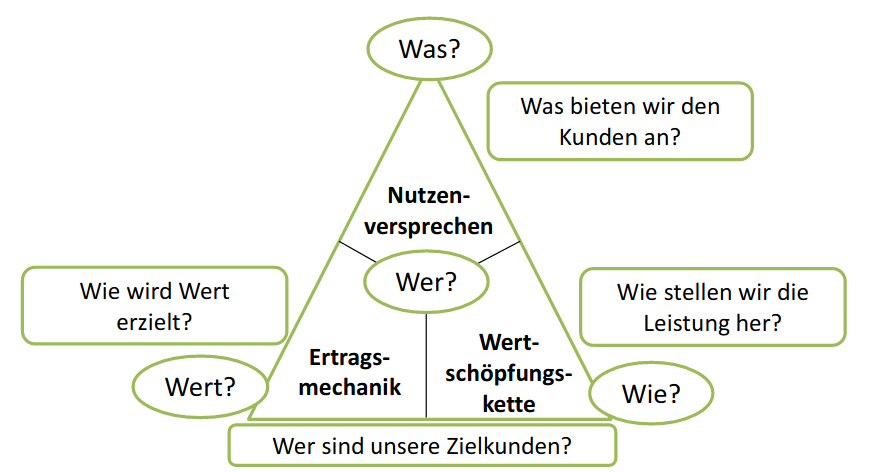
\includegraphics[scale=0.45]{wfragen.png}

\vspace*{2em}

\textbf{Geschäftsmodelltypen}

\begin{itemize}
\item \textbf{Produkt-Geschäftsmodell}
\begin{itemize}
\item standardisierte Produkte und Dienstleistungen
\item breite Kundenbasis
\item tiefe Transaktionskosten
\item Differenzierung durch Preis oder Leistung
\item Beispiel: Autos
\end{itemize}
\item \textbf{Plattform-Geschäftsmodell}
\begin{itemize}
\item gemeinsame, integrative Architektur 
\item große Bandbreite oder Tiefe oft digitaler Angebote
\item Netzwerkeffekte für die Nutzer der Plattform
\item Differenzierung über Nutzerzahlen
\item Beispiel: soziale Netzwerke
\end{itemize}
\item \textbf{Projekt-Geschäftsmodell}
\begin{itemize}
\item kundenindividuelle Produkte und Dienstleistungen
\item einmalige Leistungsvereinbarungen
\item Differenzierung durch Flexibilität
\item hoher Serviceanteil
\item Beispiel: Aufzug bauen
\end{itemize}
\item \textbf{Lösungs-Geschäftsmodell}
\begin{itemize}
\item Kombination kundenindividueller Angebote
\item integrierte End-to-End Leistungen
\item langfristige Verträge
\item gegenseitige Abhängigkeit zwischen Anbieter und Abnehmer
\item Beispiel: Logistik
\end{itemize}
\end{itemize}

\newpage

\textbf{Eigenschaften digitaler Geschäftsmodelle} \\
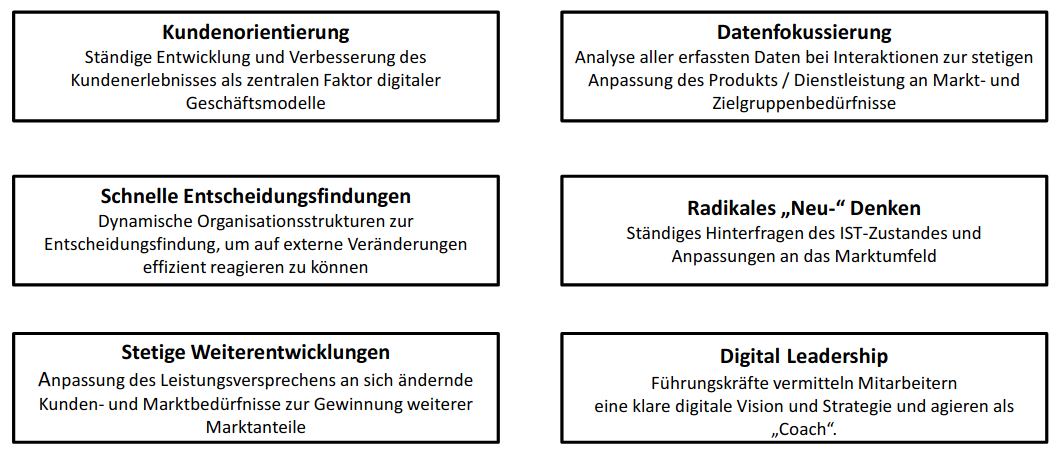
\includegraphics[scale=0.33]{edg.png} \\

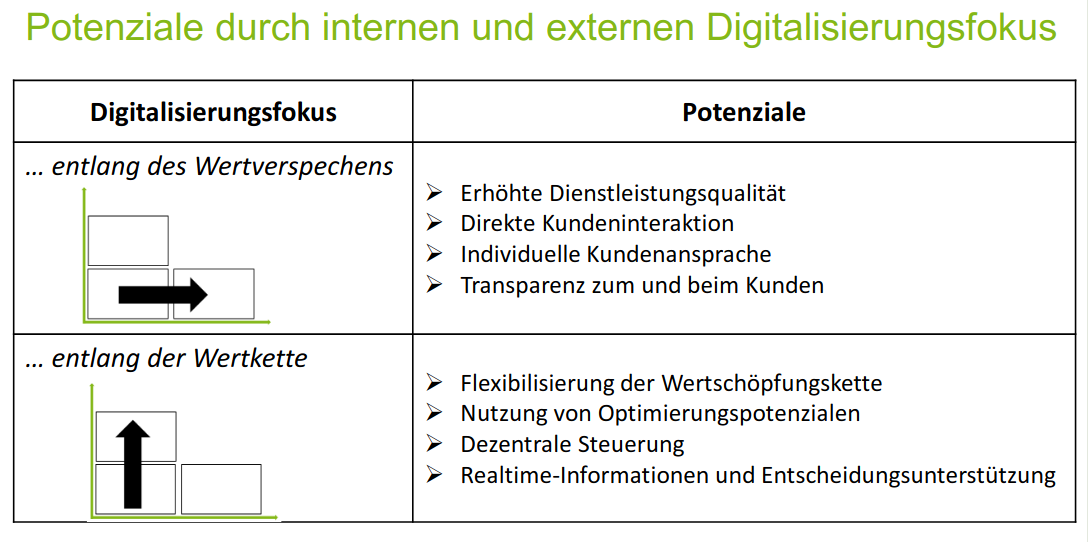
\includegraphics[scale=0.3]{potdig.png}
\\

\textbf{Häufige Geschäftsmodellmuster digitaler Unternehmen}

\begin{itemize}
\item \textbf{Freemium}
\begin{itemize}
\item kostenlose Basisversion und Premiumversion, oft als Abo-Modell
\item Beispiel: Dropbox
\end{itemize}
\item \textbf{Abonnement/Subscription}
\begin{itemize}
\item Beispiel: Netflix
\end{itemize}
\item \textbf{Add-On}
\begin{itemize}
\item Nutzen eines Services oder Produkts zu einem möglichst geringen Kaufpreis anbieten. Durch gebührenpflichtige Zusätze kann das Produkt beliebig erweitert werden. 
\item Beispiel: SAP
\end{itemize}
\item \textbf{Lock-In}
\begin{itemize}
\item Kunden werden an ein Produkt gebunden, indem die Kosten für einen Ausstieg oder Wechsel gesteigert werden.
\item Beispiel: AmazonPrime
\end{itemize}
\item \textbf{rent instead of buy}
\begin{itemize}
\item Unternehmen verkauft das Produkt nicht, sondern gewährt Kunden gegen einen kleineren Betrag zeitlich limitierte Nutzungsrechte.
\item E-Scooter leihen
\end{itemize}
\item \textbf{Plattform/mehrseitige Märkte}
\begin{itemize}
\item Unterscheidbare Nutzergruppen, werden auf der Plattform eines Dritten zusammengeführt.
\item Beispiel: Google
\end{itemize}
\end{itemize}

\newpage

\textbf{Modellierung von Geschäftsmodellen}

\begin{itemize}
\item Kernelemente und -logik eines Geschäftsmodells visualisieren
\item existierende Geschäftsmodelle besser verstehen
\item Ideen für neue, innovative Geschäftsmodelle zu generieren
\end{itemize}

\textbf{Business Model Canvas (BMC)}

\begin{itemize}
\item Kundennutzen stellt Kern dar
\item 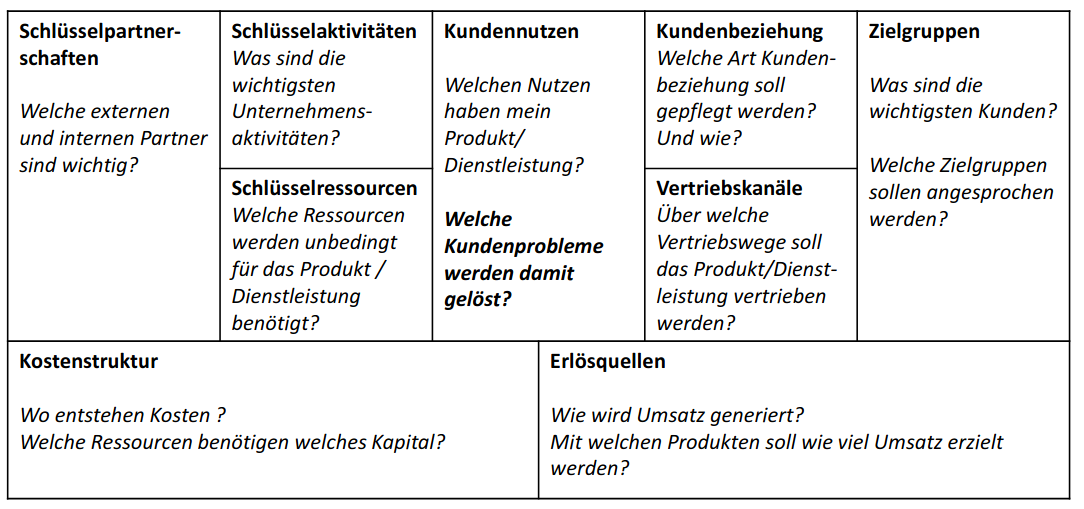
\includegraphics[scale=0.4]{BMC.png}
\end{itemize}


\textbf{e$^3$-Value Modellierung} \\
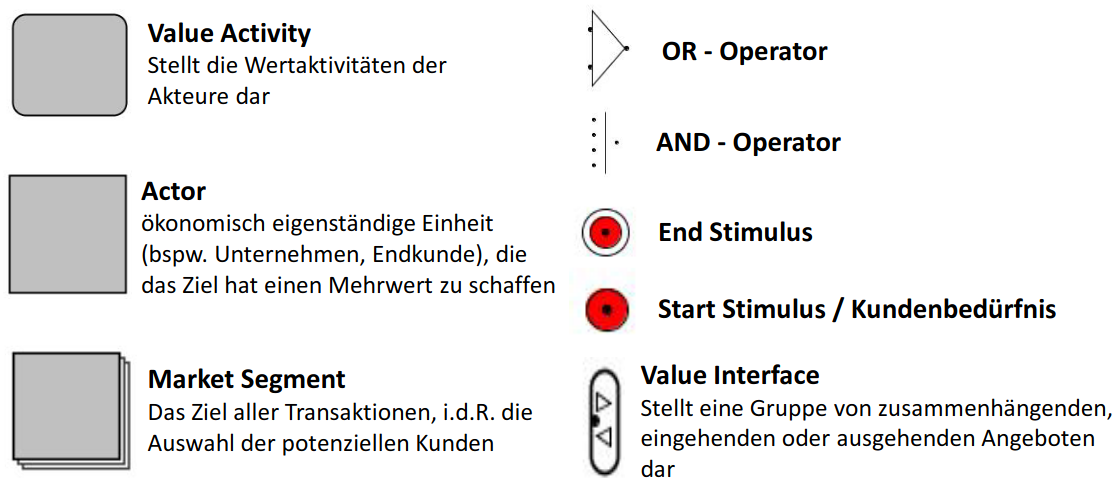
\includegraphics[scale=0.4]{modelldings.png} \\
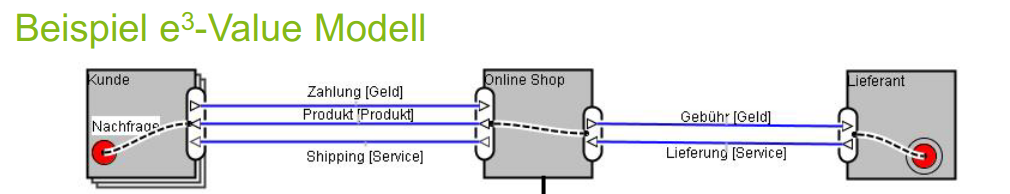
\includegraphics[scale=0.4]{beispiel_e3.png}

\newpage

\textbf{BMC vs. e$^3$-Value}

\vspace*{1em}

\adjustbox{max width=\textwidth}{%
\begin{tabular}{l l l}

 & \textbf{BMC} & \textbf{e$^3$-Value} \\
\hline
\textbf{Stärken:} & ganzes Geschäftsmodell wird beschrieben & Schnittstellen werden dargestellt \\
 & deutliche Herausstellung der Value Proposition\footnotemark & Berechnung des Wertflusses \\
 & & Nutzenanalysen pro Akteur möglich \\
 & &  \\
\textbf{ Schwächen:} & keine Darstellung d. Interaktion von Akteuren & Datenbasis muss vorhanden sein \\
 & fehlender Detaillierungsgrad & Hohe Komplexität bei größeren Netzwerken \\
 & fehlende Nutzungsbeurteilung & keine Herausstellung der Value Proposition \\
  & &  \\
\textbf{Innovationsgrad:} & bei radikalen Innovationen sinnvoll & bei inkrementellen\footnotemark Innovationen sinnvoll \\

\end{tabular}}

\footnotetext[4]{Nutzenversprechen (englisch value proposition) beschreibt, welchen Nutzen ein Unternehmen seinen Kunden mit einem bestimmten Produkt oder einer bestimmten Dienstleistung verspricht. }

\footnotetext[5]{Bei inkrementeller Innovation werden bekannte Technologien, Produkte, Dienstleistungen, Geschäftsmodelle oder Prozesse weiterentwickelt, bleiben aber im Kern erhalten.}




\end{document}






